\documentclass[12pt, a4paper, oneside, openright, titlepage]{book}
\usepackage[utf8]{inputenc}
\raggedbottom
\usepackage{import}


%%%%%%%%%%%%%%%%% Book Formatting Comments:

%%%%%%%%%%%%%%%%%%%%%%%%%%%%%%%%%%%%% for Part

%%%%%%%%%%%%%%%%%%%%%% for chapter

%%%%%%%%%%%%%%%%%%%% for section




%%%%%% PACKAGES %%%%%%%
\usepackage{hyperref}
\hypersetup{
    colorlinks,
    citecolor=black,
    filecolor=black,
    linkcolor=black,
    urlcolor=black
}
\usepackage{amsmath} % Math display options
\usepackage{amssymb} % Math symbols
%\usepackage{amsfonts} % Math fonts
%\usepackage{amsthm}
\usepackage{mathtools} % General math tools
\usepackage{array} % Allows you to write arrays
\usepackage{empheq} % For boxing equations
% \usepackage{mathabx}
% \usepackage{mathrsfs}
\usepackage{nameref}
\usepackage{wrapfig}

\usepackage{soul}
\usepackage[normalem]{ulem}

\usepackage{txfonts}
\usepackage{cancel}
\usepackage[toc, page]{appendix}
\usepackage{titletoc,tocloft}
\setlength{\cftchapindent}{1em}
\setlength{\cftsecindent}{2em}
\setlength{\cftsubsecindent}{3em}
%\setlength{\cftsubsubsecindent}{4em}
\usepackage{titlesec}

%\titleformat{\section}
%  {\normalfont\fontsize{25}{15}\bfseries}{\thesection}%{1em}{}
%\titleformat{\section}
%  {\normalfont\fontsize{20}{15}\bfseries}%{\thesubsection}{1em}{}
%\setcounter{secnumdepth}{1}  
  
  

%\newcommand\numberthis{\refstepcounter{equation}\tag{\theequation}} % For equation labelling
\usepackage[framemethod=tikz]{mdframed}

\usepackage{tikz} % For drawing commutative diagrams
\usetikzlibrary{cd}
\usetikzlibrary{calc}
\tikzset{every picture/.style={line width=0.75pt}} %set default line width to 0.75p

\usepackage{datetime}
\usepackage[margin=1.5in]{geometry}
\setlength{\parskip}{1em}
\usepackage{makeidx}         % allows index generation
\usepackage{graphicx}       % standard LaTeX graphics tool
\usepackage{multicol}        % used for the two-column index
\usepackage[bottom]{footmisc}% places footnotes at page bottom

\usepackage{newtxtext}       % 
\usepackage{newtxmath}       % selects Times Roman as basic font
\usepackage{float}
\usepackage{fancyhdr}
\setlength{\headheight}{15pt} 
\pagestyle{fancy}
\lhead[\leftmark]{}
\rhead[]{\leftmark}

%\usepackage{enumitem}

\usepackage{url}
\allowdisplaybreaks

%%%%%% ENVIRONMENTS %%%
\definecolor{purp}{rgb}{0.29, 0, 0.51}
\definecolor{bloo}{rgb}{0, 0.13, 0.80}



%%\newtheoremstyle{note}% hnamei
%{3pt}% hSpace above
%{3pt}% hSpace belowi
%{}% hBody fonti
%{}% hIndent amounti
%{\itshape}% hTheorem head fonti
%{:}% hPunctuation after theorem headi
%{.5em}% hSpace after theorem headi
%{}% hTheorem head spec (can be left empty, meaning ‘normal’)i





% %%%%%%%%%%%%% THEOREM DEFINITIONS

\spnewtheorem{axiom}{Axiom}[chapter]{\bfseries}{\itshape}


\spnewtheorem{construction}{Construction}[chapter]{\bfseries}{\itshape}

\spnewtheorem{props}{Properties}[chapter]{\bfseries}{\itshape}


\renewcommand{\qedsymbol}{$\blacksquare$}


\numberwithin{equation}{section}

\newenvironment{qest}{
    \begin{center}
        \em
    }
    {
    \end{center}
    }

%%%%%% MACROS %%%%%%%%%
%% New Commands
\newcommand{\ip}[1]{\langle#1\rangle} %%% Inner product
\newcommand{\abs}[1]{\lvert#1\rvert} %%% Modulus
\newcommand\diag{\operatorname{diag}} %%% diag matrix
\newcommand\tr{\mbox{tr}\.} %%% trace
\newcommand\C{\mathbb C} %%% Complex numbers
\newcommand\R{\mathbb R} %%% Real numbers
\newcommand\Z{\mathbb Z} %%% Integers
\newcommand\Q{\mathbb Q} %%% Rationals
\newcommand\N{\mathbb N} %%% Naturals
\newcommand\F{\mathbb F} %%% An arbitrary field
\newcommand\ste{\operatorname{St}} %%% Steinberg Representation
\newcommand\GL{\mathbf{GL}} %%% General Linear group
\newcommand\SL{\mathbf{SL}} %%% Special linear group
\newcommand\gl{\mathfrak{gl}} %%% General linear algebra
\newcommand\G{\mathbf{G}} %%% connected reductive group
\newcommand\g{\mathfrak{g}} %%% Lie algebra of G
\newcommand\Hbf{\mathbf{H}} %%% Theta fixed points of G
\newcommand\X{\mathbf{X}} %%% Symmetric space X
\newcommand{\catname}[1]{\normalfont\textbf{#1}}
\newcommand{\Set}{\catname{Set}} %%% Category set
\newcommand{\Grp}{\catname{Grp}} %%% Category group
\newcommand{\Rmod}{\catname{R-Mod}} %%% Category r-modules
\newcommand{\Mon}{\catname{Mon}} %%% Category monoid
\newcommand{\Ring}{\catname{Ring}} %%% Category ring
\newcommand{\Topp}{\catname{Top}} %%% Category Topological spaces
\newcommand{\Vect}{\catname{Vect}_{k}} %%% category vector spaces'
\newcommand\Hom{\mathbf{Hom}} %%% Arrows

\newcommand{\map}[2]{\begin{array}{c} #1 \\ #2 \end{array}}

\newcommand{\Emph}[1]{\textbf{\ul{\emph{#1}}}}




%% Math operators
\DeclareMathOperator{\ran}{Im} %%% image
\DeclareMathOperator{\aut}{Aut} %%% Automorphisms
\DeclareMathOperator{\spn}{span} %%% span
\DeclareMathOperator{\ann}{Ann} %%% annihilator
\DeclareMathOperator{\rank}{rank} %%% Rank
\DeclareMathOperator{\ch}{char} %%% characteristic
\DeclareMathOperator{\ev}{\bf{ev}} %%% evaluation
\DeclareMathOperator{\sgn}{sign} %%% sign
\DeclareMathOperator{\id}{Id} %%% identity
\DeclareMathOperator{\supp}{Supp} %%% support
\DeclareMathOperator{\inn}{Inn} %%% Inner aut
\DeclareMathOperator{\en}{End} %%% Endomorphisms
\DeclareMathOperator{\sym}{Sym} %%% Group of symmetries


%% Diagram Environments
\iffalse
\begin{center}
    \begin{tikzpicture}[baseline= (a).base]
        \node[scale=1] (a) at (0,0){
          \begin{tikzcd}
           
          \end{tikzcd}
        };
    \end{tikzpicture}
\end{center}
\fi




\newdateformat{monthdayyeardate}{%
    \monthname[\THEMONTH]~\THEDAY, \THEYEAR}
%%%%%%%%%%%%%%%%%%%%%%%

%%% Specific Macros %%%


%%%%%% BEGIN %%%%%%%%%%


\begin{document}

%%%%%% TITLE PAGE %%%%%

\begin{titlepage}
    \centering
    \scshape
    \vspace*{\baselineskip}
    \rule{\textwidth}{1.6pt}\vspace*{-\baselineskip}\vspace*{2pt}
    \rule{\textwidth}{0.4pt}
    
    \vspace{0.75\baselineskip}
    
    {\LARGE Theoretical Computer Science: A Complete Guide}
    
    \vspace{0.75\baselineskip}
    
    \rule{\textwidth}{0.4pt}\vspace*{-\baselineskip}\vspace{3.2pt}
    \rule{\textwidth}{1.6pt}
    
    \vspace{2\baselineskip}
    Computer Science \\
    \vspace*{3\baselineskip}
    \monthdayyeardate\today \\
    \vspace*{5.0\baselineskip}
    
    {\scshape\Large Elijah Thompson, \\ Physics and Math Honors\\}
    
    \vspace{1.0\baselineskip}
    \textit{Solo Pursuit of Learning}
    \vfill
    \enlargethispage{1in}
    \begin{figure}[b!]
    \makebox[\textwidth]{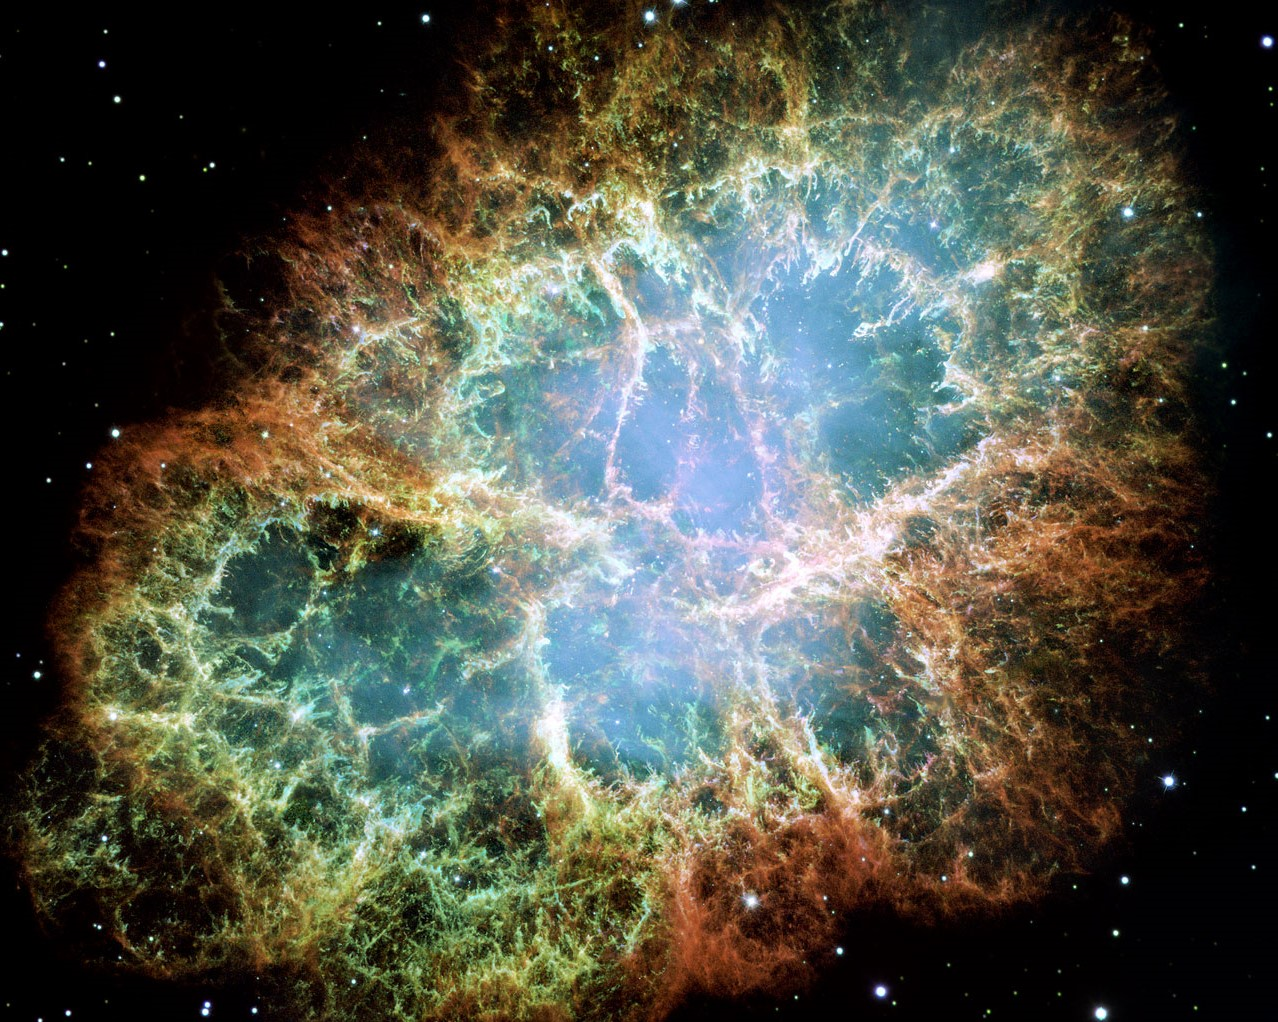
\includegraphics[width=\paperwidth, height =10cm]{../Crab.jpg}}
    \end{figure}
\end{titlepage}

%%%%%%%%%%%%%%%%%%%%%%%
\tableofcontents

%%%%%%%%%%%%%%%%%%%%%%%%%%%%%%%%%%%%% Part 1.
\part{Comp Phys 381}

%%%%%%%%%%%%%%%%%%%%%%% - Chapter 1
\chapter{Root Finding Methods}



\section{Bisection Method}

\begin{proc}
	To find the roots of a function $f$ we first choose a pair of initial values $x_B$ and $x_U$ such that $f(x_B) < 0$ and $f(x_U) > 0$. Then we perform the following iterative procedure:
	\begin{enumerate}
		\item Define $x_C = \frac{x_B+x_U}{2}$, and evaluate $f(x_C)$.
		\item If $f(x_C) > 0$ set $x_U = x_C$
		\item If $f(x_C) < 0$ set $x_B = x_C$
		\item Repeat until $|f(x_C)|$ is less than some chosen tolerance, $\epsilon$.
	\end{enumerate}
\end{proc}


\section{Newton-Raphson Method}

\begin{proc}
        Consider a real valued function $f$. Note that the Taylor expansion of $f$ centered at a point $x_0$ and evaluated at $x_0 + \epsilon$ is \begin{equation}
                f(x_0+\epsilon) = f(x_0) + f'(x_0)\epsilon + \frac{1}{2}f''(x_0)\epsilon^2 + ... = \sum_{n=0}^{\infty}\frac{f^{(n)}(x_0)\epsilon^n}{n!}
        \end{equation}
        With the NR Method $x_0$ is the current estimate for the root of our function. We now truncate the series to terms linear in $\epsilon$: \begin{equation}
                f(x_0+\epsilon) = f(x_0) + f'(x_0)\epsilon + O(\epsilon^2)
        \end{equation}
        where $O(\epsilon^2)$ indicates that the terms of order $\epsilon^2$ and higher are omitted. We set $f(x_0+\epsilon) = 0$. This gives \begin{equation}
                f(x_0) + f'(x_0)\epsilon = 0
        \end{equation}
        from which we obtain \begin{equation}
                \epsilon_0 = -\frac{f(x_0)}{f'(x_0)}
        \end{equation}
        setting $\epsilon = \epsilon_0$. We then let $x_1 = x_0 + \epsilon_0$ and calculate a new $\epsilon_1$. We extend this process and define it recursively as \begin{equation}
                x_{n+1} = x_n - \frac{f(x_n)}{f'(x_n)}
        \end{equation}
        for an indexing ineger $n \geq 0$.
\end{proc}




%%%%%%%%%%%%%%%%%%%%%%% - Chapter 2
\chapter{Non-Linear ODEs}

\begin{rmk}
        In this chapter considered the differential equation described by \begin{equation}
                \frac{dx}{dt} = y, \;\;\frac{dy}{dt} = f(x,y,t)
        \end{equation}
\end{rmk}


\section{Euler Method}

\begin{proc}
        We first choose initial conditions $x(0) = x_0$ and $y(0) = y_0$. Consider the Taylor series expansion of a function $g$ about $a+h$ centered at $a$:\begin{equation}
                f(a+h) = f(a) + hf'(a) + \frac{h^2}{2!}f''(a) + O(h^3)
        \end{equation}
        We apply this to $x(t)$ and $y(t)$ to obtain \begin{align}
                x(t + \Delta t) &= x(t) + \Delta t \frac{dx(t)}{dt} + O(\Delta t^2)\\
                y(t + \Delta t) &= y(t) + \Delta t \frac{dy(t)}{dt} + O(\Delta t^2)
        \end{align}
        where we omit terms of order $\Delta t^2$. We shall vary $t$ steps discretely and label $\Delta t = t_{n-1} - t_n$, so our equations of motion become \begin{align}
                x_{n+1} &= x_n + y_n\Delta t \\
                y_{n+1} &= y_n + f(x_n,y_n,t_n)\Delta t
        \end{align}
        using Euler's Method for approximating integrals. In particular, for Euler's method we take \begin{equation}
                g(b) - g(a) = \int_a^b\frac{dg}{dt}dt \approx \sum_{i=1}^n\frac{dg(t_i)}{dt}\Delta t, t_1 = a, t_n = b - \Delta t
        \end{equation}
\end{proc}


\section{Trapezoid Rule}


\begin{proc}
        For the trapezoid rule we approximate an integral as follows \begin{equation}
                (b-a)\left[\frac{\frac{dg(a)}{dt} + \frac{dg(b)}{dt}}{2}\right] \approx \int_a^b\frac{dg}{dt}dt = g(b) - g(a)
        \end{equation}
        Then, applying this to our DE we obtain the iterative equation \begin{equation}
                x_{n+1} \approx x_n + \frac{\Delta t}{2}\left(y_n + y_{n+1}\right)
        \end{equation}
        where $\Delta t = t_{n+1} - t_n$. We then approximate $y_{n+1}$ using Euler's Method \begin{equation}
                y_{n+1} \approx y_n + \Delta t f(x_n,y_n, t_n)
        \end{equation}
        Substituting this back into our previous approximation for $x_{n+1}$ we have \begin{equation}
                x_{n+1} \approx x_n + \frac{\Delta t}{2}\left[y_n + (y_n + \Delta tf(x_n,y_n,t_n)\right]
        \end{equation}
        We apply this again to $y_{n+1}$ to obtain the approximation \begin{equation}
                y_{n+1} \approx y_n + \frac{\Delta t}{2}\left[f(x_n,y_n,t_n) + \delta tf(x_{n+1},y_n + \Delta tf(x_n,y_n,t_n), t_{n+1})\right]
        \end{equation}
        This pair of iterative equations constitute the application of the trapezoid rule to solving our DE.
\end{proc}


\section{Runge-Kutta}


\begin{proc}[Second Order]
        We first carry out a Taylor expansion of $\frac{dx(t)}{dt}$ about the midpoints of our interval, $\Delta t/2$: \begin{equation}
                \frac{dx(t)}{dt} = \frac{dx(\Delta t/2)}{dt} + \frac{d^2x(\Delta t/2)}{dt^2}(t - \Delta t/2) + O\left(\frac{\Delta t}{2}^2\right)
        \end{equation}
        We use this expansion to approximate the following integral:\begin{equation}
                \int_{0}^{\Delta t}\frac{x(t)}{dt}dt \approx \frac{dx(\Delta t/2)}{dt}\Delta t + \frac{d^2x(\Delta t/2)}{dt^2}\int_{0}^{\Delta t}(t-\Delta t/2)dt = \frac{dx(\Delta t/2)}{dt}\Delta t
        \end{equation}
        Then, the rule to update $x$ in an algorithmic notation is given by \begin{equation}
                x_{n+1} \approx x_n + y_{n+1/2}\Delta t + O\left(\frac{\Delta t}{2}^2\right)
        \end{equation}
        and applying the Taylor expansion to $y_{n+1/2}$ we have \begin{equation}
                y_{n+1/2} \approx = y_n + f(x_n,y_n,t_n)\frac{\Delta t}{2} + O\left(\frac{\Delta t}{2}^2\right)
        \end{equation}
        Substituing into our $x_{n+1}$ rule we have \begin{equation}
                x_{n+1} \approx x_n + \left( y_n + f(x_n,y_n,t_n)\frac{\Delta t}{2}\right)\Delta t
        \end{equation}
        The rule for updating $y_n$ is given by \begin{align}
                y_{n+1} &= y_n + f(x_{n+1/2},y_{n+1/2},t_{n+1/2})\Delta t \\
                y_{n+1/2} &= y_n + f(x_n,y_n,t_n)\frac{\Delta t}{2} \\
                x_{n+1/2} &= x_n + y_n\frac{\Delta t}{2} 
        \end{align}
\end{proc}


\begin{proc}[Fourth Order]
        In implementing we take a series of approximations for $x_n$ and $y_n$ then take a weighted average of the result. In particular, we take the approximations \begin{align}
                k_{1x,n} &= \Delta t y_n \\
                k_{1y,n} &= \Delta t f(x_n,y_n,t_n) \\
                k_{2x,n} &= \Delta t \left(y_n+ \frac{k_{1y,n}}{2}\right) \\
                k_{2y,n} &= \Delta tf\left(x_n + \frac{k_{1x,n}}{2}, y_n + \frac{k_{1y,n}}{2}, t_n + \Delta t/2\right) \\
                k_{3x,n} &= \Delta t\left(y_n+ \frac{k_{2y,n}}{2}\right) \\
                k_{3y,n} &= \Delta t f\left(x_n + \frac{k_{2x,n}}{2}, y_n + \frac{k_{2y,n}}{2}, t_n + \Delta t/2\right) \\
                k_{4x,n} &= \Delta t \left(y_n + k_{3y,n}\right)\\
                k_{4y,n} &= \Delta tf\left(x_n + k_{3x,n}, y_n + k_{3y,n}, t_n + \Delta t\right) \\
                x_{n+1} &= x_n + \frac{k_{1x,n} + 2k_{2x,n} + 2k_{3x,n} + k_{4x,n}}{6} \\
                y_{n+1} &= y_n + \frac{k_{1y,n} + 2k_{2y,n} + 2k_{3y,n} + k_{4y,n}}{6} 
        \end{align}
\end{proc}






%%%%%%%%%%%%%%%%%%%%%%% - Chapter 3
\chapter{Numerical Fourier Analysis}


\section{Fourier Series}


\begin{defn}[Fourier Series]
        Any periodic function $f(t)$ with period $T = 2\pi/\omega$ can be represented as a \Emph{Fourier Series}\begin{equation}
                f(t) = a_0 + \sum_{n=1}^{\infty}\left[a_n\cos(n\omega t) + b_n\sin(n\omega t)\right]
        \end{equation}
        The frequency $\omega$ is known as the \Emph{fundamental frequency} and $\omega_n = n\omega$ for $n >1$ are the \Emph{harmonics}. The result of Fourier-analysing a signal is a set of values for these coefficients for all $n$.
\end{defn}

\begin{proc}
        The Fourier coefficients for a periodic function $f$ are evaluated using the orthogonality properties of sines and cosines:\begin{align}
                \frac{2}{T}\int_0^T\sin(n\omega t)\sin(k\omega t)dt &= \delta_{nk} \\
                \frac{2}{T}\int_0^T\cos(n\omega t)\sin(k\omega t)dt &= 0 \\
                \frac{2}{T}\int_0^T\cos(n\omega t)\cos(k\omega t)dt &= \delta_{nk}
        \end{align}
        Applying these orthogonality properties we obtain the following equations for the coefficients:\begin{align}
                a_0 &= \frac{1}{T}\int_0^Tf(t)dt \\
                a_k &= \frac{2}{T}\int_0^Tf(t)\cos(k\omega t)dt, k \in \{1,2,3,...\} \\
                b_k &= \frac{2}{T}\int_0^Tf(t)\sin(k\omega t)dt, k\in \{1,2,3,...\}
        \end{align}
\end{proc}


\section{Simpson's Rule}

\begin{proc}
        Simpson's rule is a method of numerical integration. In particular, to approximate the integral $\int_a^bf(x)dx$ we split the interval $[a,b]$ into $n$ steps of length $h = (b-a)/n$, where $n \in 2\Z$. The approximation is taken as \begin{equation}
                \int_a^bf(t)dt \approx \frac{h}{3}\left[ f(x_0) + 2\sum_{j=1}^{n/2-1}f(x_{2j}) + 4\sum_{j=1}^{n/2}f(x_{2j-1}) + f(x_n)\right]
        \end{equation}
        where $x_j = a + jh$ for $j \in \{0,1,2,...,n-1, n\}$. In particular $x_0 = a$ and $x_n = b$.
\end{proc}


\section{Fourier Integral}

\begin{rmk}
        For a non-periodic function $f(t)$ we require a \Emph{Fourier integral} over a continuous range of frequencies. The Fourier integral may be viewed as a limit of a Fourier series in the limit $T\rightarrow \infty$.
\end{rmk}


\begin{proc}
        For a non periodic function $f(t)$ its Fourier integral is given by \begin{equation}
                f(t) = \int_0^{\infty}\left[a(\omega)\cos(\omega t) + b(\omega)\sin(\omega t)\right]d\omega
        \end{equation}
        and the coefficient equations become functions of $\omega$:\begin{align}
                a(\omega) &= \frac{1}{\pi}\int_{-\infty}^{\infty}f(t)\cos(\omega t)dt \\
                b(\omega) &= \frac{1}{\pi}\int_{-\infty}^{\infty}f(t)\sin(\omega t)dt
        \end{align}
        Using Euler's identity $e^{i\omega t} = \cos(\omega t) + i\sin(\omega t)$ we can rewrite this as \begin{align}
                f(t) &= \frac{1}{\sqrt{2\pi}}\int_{-\infty}^{\infty}F(\omega)e^{i\omega t}d\omega \\
                F(\omega) &= \frac{1}{\sqrt{2\pi}}\int_{-\infty}^{\infty}f(t)e^{-i\omega t}dt
        \end{align}
        where $F(\omega)$ is the \Emph{Fourier Transform} of $f(t)$. If the signal has dimensions of energy, then its Fourier Transform has units of Power, and its magnitude $|F(\omega)|$ is a measure of the total power in the signal at frequency $\omega$: \begin{equation}
                |F(\omega)| = \sqrt{\R e\{F(\omega)\}^2+\mathbb{I}m\{F(\omega)\}^2} = \sqrt{\pi}{2}\sqrt{a^2(\omega) + b^2(\omega)}
        \end{equation}
\end{proc}


\section{Discrete Fourier Transform}

\begin{defn}
        In practice we approximate the Fourier integral and its other corresponding forms using finite summations, known as the \Emph{Discrete Fourier Transform}. Let $f(t)$ be a non-periodic function that we have $N$ samples of at intervals $h$ going from $t = 0$ to $t = (N-1)h$. We define a discrete timeline by $t_m = mh$ for $m \in \{0,1,2,...,N-1\}$. The time $\tau = Nh$ will become the period of our approximated function under reconstruction, and we need $\tau$ to be the longest time over which we are interested in the behaviour of $f(t)$. We also assume \begin{equation}
                f(t) = f(t+\tau) \iff f(t_m) = f(t_{m+N}) \iff f_m = f_{m+N}
        \end{equation}
        The lowest frequency in the DFT will be $\nu_1 = 1/\tau = 1/(Nh)$, and this will be the fundamental frequency of our reconstructed function. The frequency spectrum is given by \begin{equation}
                \Lambda := \left\{\nu_n = \frac{n}{Nh} = n\nu_1\vert n \in \N\right\}
        \end{equation}
        We then discretize the integrals for the function and its Fourier transform as \begin{align}
                f_m &= frac{1}{N}\sum_{n=0}^{N-1}F_ne^{i2\pi\nu_nt_m} = \frac{1}{N}\sum_{n=0}^{N-1}F_ne^{i2\pi mn/N} \\
                F_n &= \sum_{m=0}^{N-1}f_me^{-i2\pi\nu_nt_m} = \sum_{m=0}^{N-1}f_me^{-2\pi mn/N}
        \end{align}
        Note that it can be shown that $F_{N/2-n} = \overline{F}_{N/2+n}$ for $n \in \{0,1,...,N/2\}$. The highest frequency component is thus $F_{N/2-1}$, corresponding to a frequency of \begin{equation}
                \nu_{max} = (N/2-1)/Nh = 1/(2h) - 1/(Nh) \approx 1/(2h), \text{ if $N$ large}
        \end{equation}
        This is also known as the \Emph{nyquist frequency} $\nu_{Nyquist}$.


        If the function has a component with frequency $\nu > \nu_{Nyquist}$ there are less than two sample points per period. This implies that there will be one or more frequencies less than $\nu_{Nyquist}$ for which the amplitude equals the true amplitude at the sample points, but these lower frequencies are not in the signal although they will appear in the frequency spectrum - this is phenomenon known as \Emph{aliasing}. The power spectrum of the DFT is often plotted as all values \begin{equation}
                P_n = |F_n|^2 = \R e\{F_n\}^2+\mathbb{I}m\{F_n\}^2
        \end{equation}
\end{defn}


\begin{proc}
        In application we use the following summations for the components of $F_n$ \begin{align}
                \R e\{F_n\} &= \sum_{m=0}^{N-1}f_m\cos\left(\frac{2\pi mn}{N}\right) \\
                \mathbb{I}m\{F_n\} &= \sum_{m=0}^{N-1}f_m\sin\left(\frac{2\pi mn}{N}\right)
        \end{align}
        We then reconstruct the original signal as \begin{equation}
                f_m = \frac{1}{N}\sum_{n=0}^{N-1}\left\{\R e\{F_n\}\cos\left(\frac{2\pi mn}{N}\right) + \mathbb{I}m\{F_n\}\sin\left(\frac{2\pi mn}{N}\right)\right\}
        \end{equation}
\end{proc}




%%%%%%%%%%%%%%%%%%%%%%% - Chapter 4
\chapter{Curve-fitting and Optimization}


\section{Least Squares}

\begin{proc}
        Assume we have some sequence of measurements at times $t_i$ \begin{equation}
                y_i = y(t_i)
        \end{equation}
        and for some presumed model of the relationship \begin{equation}
                ~y = f(t;p)
        \end{equation}
        expressed in terms of the independent variable $t$ and the model parameters $p$. We define the distance between a data point and our model by \begin{equation}
                \delta_i = y_i - ~y_i
        \end{equation}
        A general measure of the distance is \begin{equation}
                \sum_i|\delta_i|^d
        \end{equation}
        For $d = 2$ we obtain the \Emph{chi-squared} measure \begin{equation}
                \chi^2 = \sum_i|y_i - ~y_i(p_1,...,p_K)|^2
        \end{equation}
        The best fit is assumed to minimize $\chi^2$ with respect to the model parameters \begin{equation}
                \frac{\partial \chi^2}{\partial p_l} = \sum_i2|y_i - ~y_i(p_1,...,p_K)|\frac{\partial ~y_i}{\partial p_l}
        \end{equation}
        We also usually use the \Emph{reduce chi-squared} value \begin{equation}
                \chi^2_N = \frac{\chi^2}{N}
        \end{equation}
        In general we want $\chi^2$ to scale with the uncertainty in our measurements, so we wish to minimize \begin{equation}
                \sum\left(\frac{expected-observed}{uncertainty}\right)^2
        \end{equation}
\end{proc}

\begin{rmk}
        This minimization can be done numerically using \Emph{scipy.optimize} package's \Emph{minimize} method. This package also has a \Emph{curve\_fit} method for non-linear data sets.
\end{rmk}

\section{Finite Differences}


\begin{proc}
        Consider a real-valued function $f(x)$ and its Taylor series about some point $x=a$:\begin{equation}
                f(x) = \sum_{n=0}^{\infty}\frac{f^{(n)}(a)}{n!}(x-a)^n
        \end{equation}
        Consider a set of points, $x_i$, such that $x_{i+1} = x_i + \Delta$. Then we have that \begin{equation}
                f(x_{i+n}) = f(x_i) + f'(x_i)n\Delta + \frac{f''(x_i)}{2!}(n\Delta)^2+\frac{f'''(x_i)}{3!}(n\Delta)^3+O(\Delta^4)
        \end{equation}
        Define $f(x_{i+n}) =: f_{i+n}$. Then for neighboring points we have \begin{align}
                f_{i+1} = f_i+f'_i\Delta +\frac{f''_i}{2!}\Delta^2 + \frac{f_i'''}{3!}\Delta^3 + O(\Delta^4) \\
                f_i = f_i \\
                f_{i-1} = f_i-f'_i\Delta +\frac{f''_i}{2!}\Delta^2 - \frac{f_i'''}{3!}\Delta^3 + O(\Delta^4)
        \end{align}
        Subtracting the expression for two neighboring points we have \begin{equation}
                f_{i+1} - f_i = f'_i\Delta +\frac{f''_i}{2!}\Delta^2 + \frac{f_i'''}{3!}\Delta^3 + O(\Delta^4)
        \end{equation}
        Dividing by $\Delta$ we obtain the following \Emph{forward difference} estimate of the first derivative \begin{equation}
                \frac{f_{i+1} - f_i}{\Delta} = f'_i+\frac{f''_i}{2!}\Delta + \frac{f_i'''}{3!}\Delta^2 + O(\Delta^3) \approx f'_i + O(\Delta)
        \end{equation}
        Similarly we obtain the \Emph{backward difference} estimate \begin{equation}
                f'_i \approx \frac{f_i - f_{i-1}}{\Delta} + O(\Delta)
        \end{equation}
        We can also cancel all even terms in the expansion by \begin{equation}
                f_{i+1} - f_{i-1} = 2f'_i\Delta +2\frac{f'''_i}{3!}\Delta^3+O(\Delta^5)
        \end{equation}
        which gives us the \Emph{centered difference} estimate \begin{equation}
                f'_i \approx \frac{f_{i+1} - f_{i-1}}{2\Delta} + O(\Delta^2)
        \end{equation}
        By adding terms we can cancel all odd terms and obtain \begin{equation}
                f_{i+1} + f_{i-1} = 2f_i + 2\frac{f''_i}{2!}\Delta^2 + O(\Delta^4)
        \end{equation}
        We then obtain an expression for the \Emph{second difference} estimate \begin{equation}
                f''_i = \frac{f_{i+1} - 2f_i + f_{i-1}}{\Delta^2} + O(\Delta^2)
        \end{equation}
\end{proc}





\begin{appendices}
        \section{Lambda Functions}

        \begin{defn}
                Lambda functions are in practice one-line functions which cannot contain commands or more than one expression. In particular, a Lambda function can be created to and assigned to a variable in Python by \begin{equation}
                        g = \mathbf{lambda}\;args_{array}:function\;rule
                \end{equation}
        \end{defn}


        \section{List Comprehension}

        \begin{defn}
                List comprehension is a method of defining and filling a list all in one step. In general, list comprehension can be implemented in Python by \begin{equation}
                        list = [item\;for\;item\;in\;old\;list\;if\;P(item) == True]
                \end{equation}
        \end{defn}

        \section{ODE-int Solve}

        \begin{defn}
                The \Emph{scipy.integrate.odeint} method can be used to numerically solve a system of differential equations. Define a method which takes the input vector of the system, a timeline, as well as any other needed parameters. Then, implement odeint by \begin{equation}
                        result = odeint(system\_function, y0, t, args = (arg\_tuple))
                \end{equation}
                where $y0$ is an initial state vector.
        \end{defn}
\end{appendices}




%%%%%%%%%%%%%%%%%%%%%% - Appendices
\begin{appendices}


\end{appendices}


\end{document}


%%%%%% END %%%%%%%%%%%%%
